\ffigbox[\FBwidth]{%
\caption{\centering Graphe biparti \(H_{(E, P)}'\) après rajout de \(E_3' P_6\) dans le couplage}\label{Fig:exam_blanc_ex_4_8}
}{
    \fbox{
        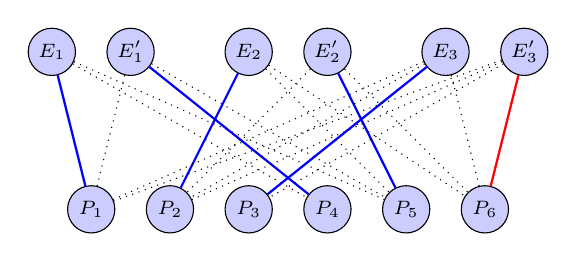
\begin{tikzpicture}[scale=1, main node/.style={circle, draw, fill=blue!20, inner sep=1pt, font=\scriptsize, minimum size=6mm}]
            % les sommets initiaux
            \node[main node] (E1) at (-3,2) {\(E_1\)};
            \node[main node] (E1p) at (-2,2) {\(E_1'\)};
            \node[main node] (E2) at (-0.5,2) {\(E_2\)};
            \node[main node] (E2p) at (0.5,2) {\(E_2'\)};
            \node[main node] (E3) at (2,2) {\(E_3\)};
            \node[main node] (E3p) at (3,2) {\(E_3'\)};
            
            \node[main node] (P1) at (-2.5,0) {\(P_1\)};
            \node[main node] (P2) at (-1.5,0) {\(P_2\)};
            \node[main node] (P3) at (-0.5,0) {\(P_3\)};
            \node[main node] (P4) at (0.5,0) {\(P_4\)};
            \node[main node] (P5) at (1.5,0) {\(P_5\)};
            \node[main node] (P6) at (2.5,0) {\(P_6\)};

            % les aretes
            \draw[draw=blue, thick] (E1) -- (P1);
            \draw[dotted] (E1) -- (P4);
            \draw[dotted] (E1) -- (P5);

            \draw[dotted] (E1p) -- (P1);
            \draw[draw=blue, thick] (E1p) -- (P4);
            \draw[dotted] (E1p) -- (P5);

            \draw[draw=blue, thick] (E2) -- (P2);
            \draw[dotted] (E2) -- (P5);
            \draw[dotted] (E2) -- (P6);

            \draw[dotted] (E2p) -- (P2);
            \draw[draw=blue, thick] (E2p) -- (P5);
            \draw[dotted] (E2p) -- (P6);

            \draw[dotted] (E3) -- (P1);
            \draw[dotted] (E3) -- (P2);
            \draw[draw=blue, thick] (E3) -- (P3);
            \draw[dotted] (E3) -- (P6);

            \draw[dotted] (E3p) -- (P1);
            \draw[dotted] (E3p) -- (P2);
            \draw[dotted] (E3p) -- (P3);
            \draw[draw=red, thick] (E3p) -- (P6);
        \end{tikzpicture}
    }
}